\documentclass[border=10pt]{standalone}

\usepackage{tikz}
\usepackage{tikzsymbols}
\usetikzlibrary{calc,patterns,shapes.geometric}

\def\centerarc[#1](#2)(#3:#4:#5){\draw[#1] ($(#2)+({#5*cos(#3)},{#5*sin(#3)})$) arc (#3:#4:#5);}

\begin{document}
	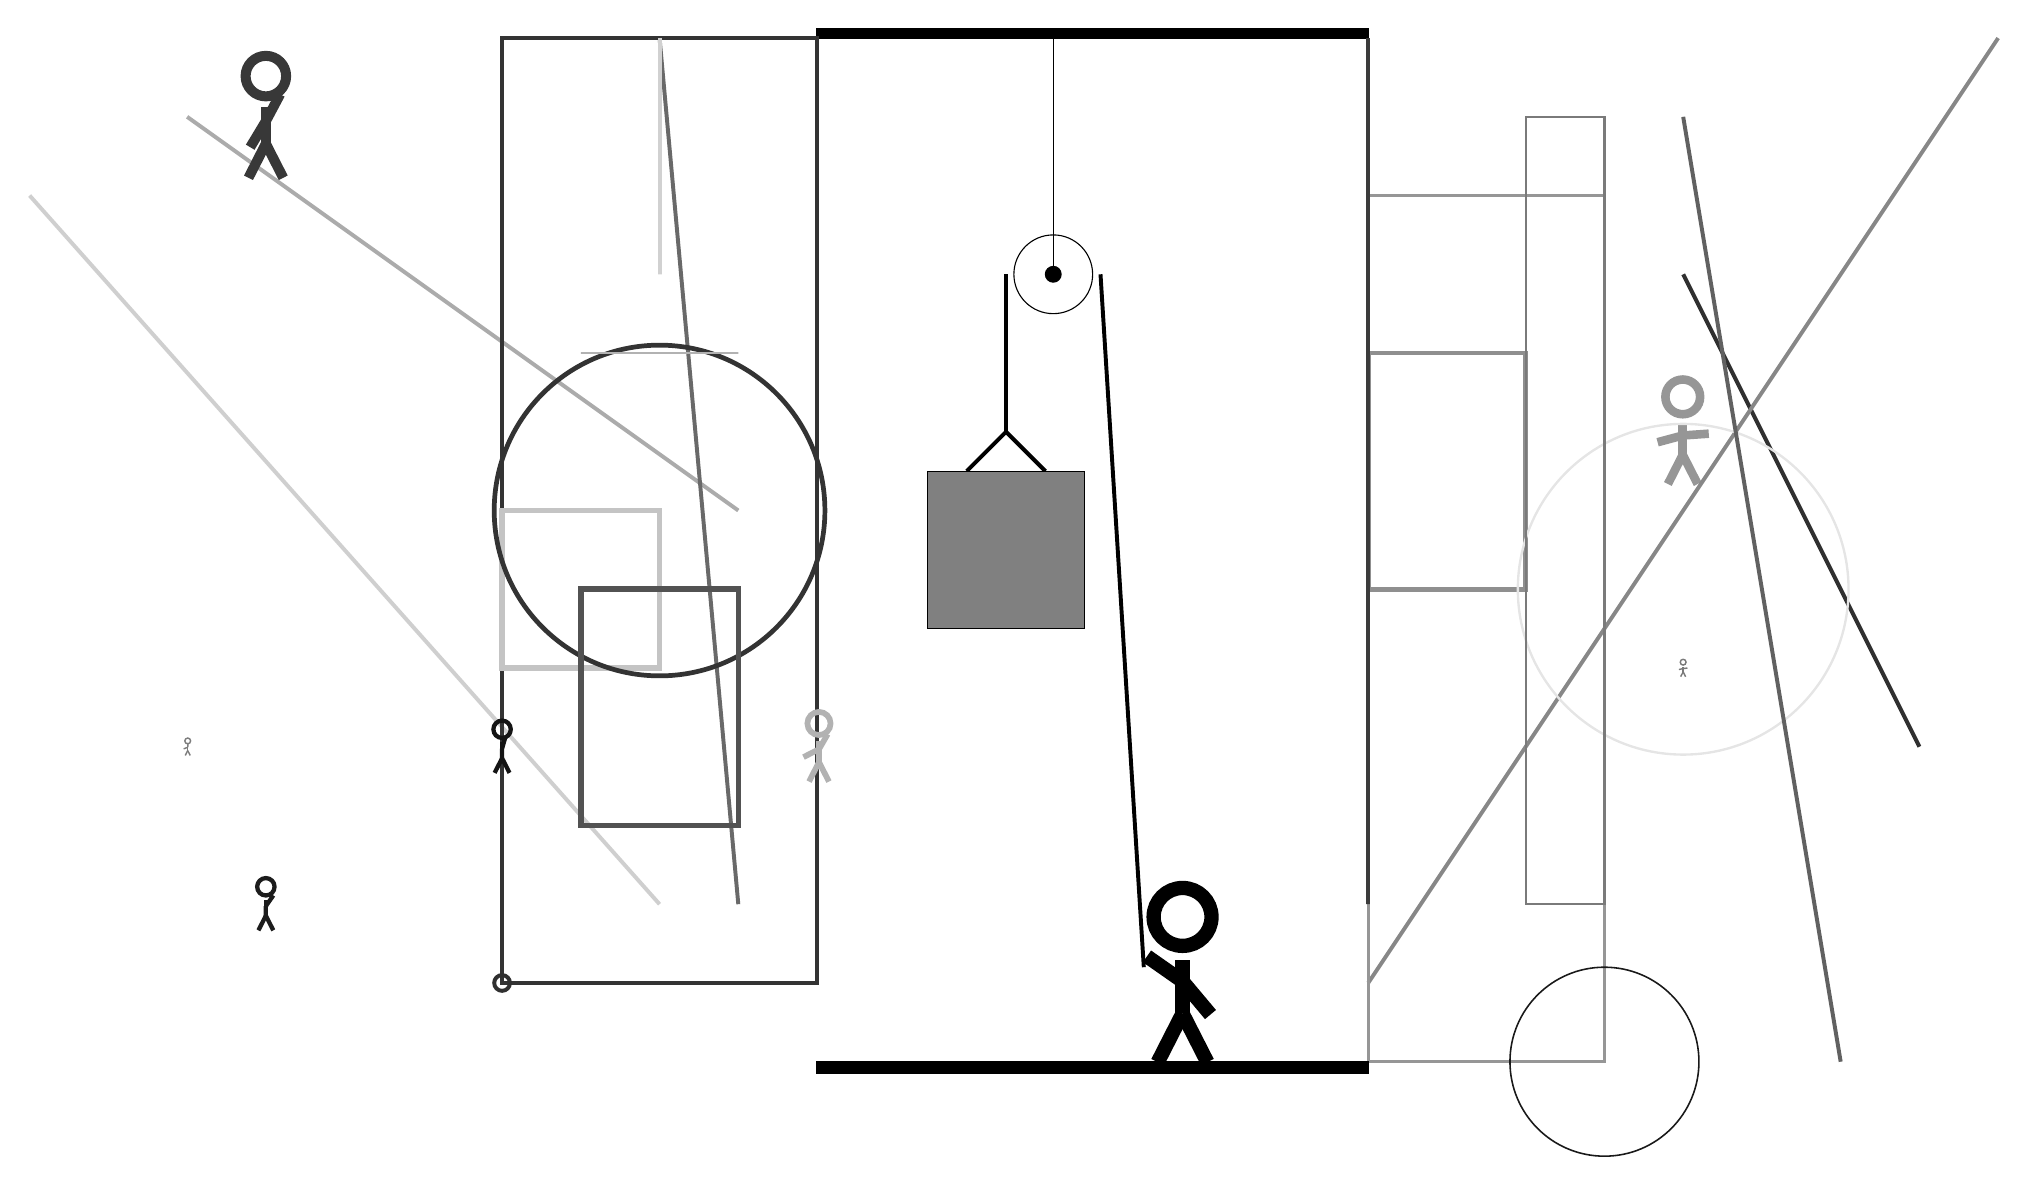
\begin{tikzpicture}
		%%%%% START %%%%%
		
		\draw[fill=black] (-2, 10) rectangle (5, 10.125);
		
		\draw (1, 7) circle (0.5);
		\draw[fill=black] (1, 7) circle (0.1);
		\draw (1, 10) -- (1, 7);
		
		\draw[line width=0.5mm, color=black!19](-4, -1) -- (-12, 8);
		
		\draw[line width=0.5mm, color=black!33](-3, 4) -- (-10, 9);
		\draw[line width=0.6mm, color=black!44] (7, 6) rectangle (5, 3);
		\draw[line width=0.5mm, color=black!81](9, 7) -- (12, 1);
		\draw[line width=0.5mm, color=black!59](-4, 10) -- (-3, -1);
		
		\node[line width=0.3mm, color=black!89] at (-9, -1) {\Strichmaxerl[3][89][55]};
		\node[line width=0.4mm, color=black!41] at (9, 5) {\Strichmaxerl[6][15][4]};
		\draw[line width=0.5mm, color=black!47](5, -2) -- (13, 10);
		\draw[line width=0.4mm, color=black!41] (5, 8) rectangle (8, -3);
		\draw [line width=0.3mm, color=black!10](9, 3) circle (2.1);
		
		\draw[line width=0.5mm, color=black!80] (-2, -2) rectangle (-6, 10);
		\draw[line width=0.7mm, color=black!23] (-4, 4) rectangle (-6, 2);
		\draw [line width=0.6mm, color=black!80](-4, 4) circle (2.1);
		
		\draw[line width=0.3mm, color=black!52] (7, 9) rectangle (8, -1);
		\node[line width=0.5mm, color=black!30] at (-2, 1) {\Strichmaxerl[4][27][60]};
		\draw [line width=0.2mm, color=black!90](8, -3) circle (1.2);
		\node[line width=0.3mm, color=black!92] at (-6, 1) {\Strichmaxerl[3][89][74]};
		
		\draw[line width=0.7mm, color=black!68] (-3, 3) rectangle (-5, 0);
		\draw[line width=0.2mm, color=black!30] (-3, 6) rectangle (-5, 6);
		\node[line width=0.6mm, color=black!52] at (9, 2) {\Strichmaxerl[1][12][8]};
		\draw[line width=0.5mm, color=black!62](9, 9) -- (11, -3);
		\draw [line width=0.5mm, color=black!81](-6, -2) circle (0.1);
		
		\draw[line width=0.5mm, color=black!77] (5, 10) rectangle (5, -1);
		\node[line width=0.2mm, color=black!78] at (-9, 9) {\Strichmaxerl[7][59][62]};
		\node[line width=0.6mm, color=black!51] at (-10, 1) {\Strichmaxerl[1][20][85]};
		
		\draw[line width=0.5mm, color=black!18] (-4, 7) rectangle (-4, 10);
		
		\draw[line width=0.5mm] (-0.1, 4.5) -- (0.4, 5.0) -- (0.9, 4.5);
		\draw[fill=black!50] (-0.6, 4.5) rectangle (1.4, 2.5);
		
		\draw[line width=0.5mm] (0.4, 7) -- (0.4, 5.0);
		\centerarc[line width=0.5mm](1, 7)(0:180:0.6);
		\draw[line width=0.5mm](1.6, 7) -- (2.15, -1.8);
		
		\node at (2.6, -1.9) {\Strichmaxerl[10][-35][-50]};
		
		\draw[fill=black] (-2, -3) rectangle (5, -3.15);
		
		%%%%% END %%%%%
	\end{tikzpicture}
\end{document}